\documentclass[a4paper]{article}
\usepackage[utf8]{inputenc}
\usepackage[russian,english]{babel}
\usepackage[T2A]{fontenc}
\usepackage[left=10mm, top=20mm, right=18mm, bottom=15mm, footskip=10mm]{geometry}
\usepackage{indentfirst}
\usepackage{amsmath,amssymb}
\usepackage[italicdiff]{physics}
\usepackage{graphicx}
\graphicspath{{images/}}
\DeclareGraphicsExtensions{.pdf,.png,.jpg}
\usepackage{wrapfig}
\usepackage{pgfplots}

\usepackage{caption}
\captionsetup[figure]{name=Рисунок}
\captionsetup[table]{name=Таблица}


\title{\underline{Лабораторная работа 2.2.3}}
\author{Старостин Александр, Б01-401}
\date {26 Марта, 2025 год}


\begin{document}

\maketitle
\newpage

\textbf{Определение теплопроводимости газов при атмосферном давлении}

\section{Аннотация}
    \par \textbf{Цель работы:} определение коэффициента теплопроводности воздуха при атмосферном давлении и разных температурах по теплоотдаче нагреваемой током нити в цилиндрическом сосуде.  \\

    \par \textbf{В работе используются:} прибор для опредления теплопроводности газов; форвакуумный насос; газгольдер с газом; манометр; магазин сопротивлений; эталонное сопротивление 10 Ом; цифровой вольтметр B7-78/1; источник питания.

\section{Теоретические сведения}

          Основной характеристикой теплопроводности служит коэффициент $\varkappa$, являющийся коэффициентом пропорциональности между плотностью потока тепла $q$ и градиентом температуры $dT/dr$ в направлении распространения этого потока
\begin{equation}
	q = -\varkappa \frac{dT}{dr}.
\end{equation}

	В цилиндрически симметричной установке, в которой тепловой поток направлен к стенкам цилиндра от нити, полынй поток тепла $Q = qS$ через каждую цилиндрическую поверхность радиуса $r$ должен в стационарном состоянии быть неизменен (как в пространстве, так и во времени). Тогда
\begin{equation}
	Q = -2\pi rL\varkappa \frac{dT}{dr} = const,
\end{equation}
откуда получаем формулу
\begin{equation}
	\label{formula}
	T_1 - T_2 = \frac{Q}{2\pi L\varkappa} \ln \frac{r_2}{r_1}.
\end{equation}
Здесь $r_1$ и $T_1$ -- радиус и температура нити, $r_2$ и $T_2$ -- радиус и температура цилиндра.



\section{Ход работы}

\subsection{Предварительные расчёты параметров установки}

$L = 0.4 \text{ м}$, \\

$\frac{r_2}{r_1} = \frac{7 \cdot 10^{-3}}{50 \cdot 10^{-6}}$. \\

Из (3) получаем ($k=\varkappa$):\\

\[Q = \frac{2\pi L k (T_1 - T_2)}{ln(\frac{r_2}{r_1})}\].

Взяв значения из методички, оценим $Q_{max}$:

\[Q_{max} = \frac{2\cdot3,14 \cdot 0,4 \text{ м} \cdot 0,025 \frac{\text{Вт}}{\text{м} \cdot K} \cdot 30 K}{ln(\frac{7 \cdot 10^{-3}}{50 \cdot 10^{-6}})} = 0.38 \text{ Дж} \].

Известно, что:

\[I^2R = Q\],
\[I_{max} = \sqrt{\frac{Q_{max}}{R}} = \sqrt{\frac{0.38 \text{Дж}}{20 \text{ Ом}}} = 138 \text{ мA}\].

Тк на каждой температуре мы будем производить по 10 измерений сил тока и напряжения на проволке, то сила тока будет изменяться в пределах от 0 до 138 $\text{ мА}$ c шагом  10-13.8 $\text{ мА}$. \\

\subsection{Подготовка установки}

Необходимо установить сопротивление на мосту сопротивлений >10 $\text{ кОм}$, чтобы сила тока через проволку была равна 0, проверить цепь, настроить вольметр и амперметр, включить источник питания и термостат. Температура в термостате в начальный момент равны комнатной. Во время всех измерений температура на термостате должна быть неизменной.

\subsection{Проведение измерений}

Для 5 температур в диапозоне от 20 до 80 $C^\circ$ проведём 10 измерений сил тока и напряжения на проволке и с помощью этих данных вычислим значения сопротивления проволки и количетсва теплоты, выделяемого проволкой при проходе через неё тока. \\

\[R = \frac{U}{I}\], & \[Q = UI\].

Таблицы с измерениями: \\

При $t = 23C^\circ$:
\begin{figure}[ht]
    \centering
    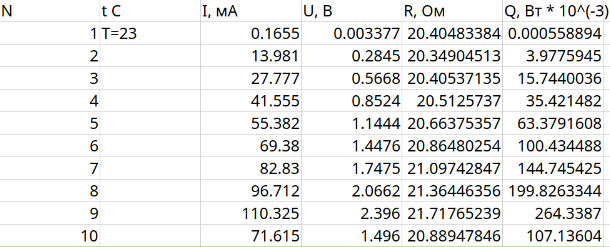
\includegraphics[width=0.6\textwidth]{tables/T23.png}
    \caption{Таблица с данными при $t = 23C^\circ$}
    %\label{plot:T_cool_3}
\end{figure}

При $t = 30C^\circ$:
\begin{figure}[ht]
    \centering
    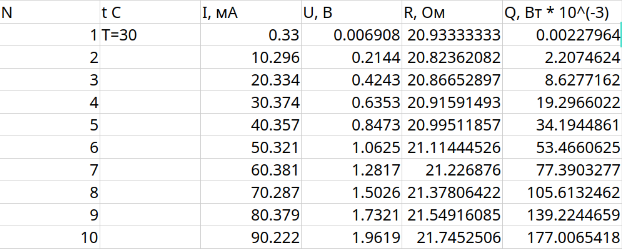
\includegraphics[width=0.6\textwidth]{tables/T30.png}
    \caption{Таблица с данными при $t = 30C^\circ$}
\end{figure}

При $t = 50C^\circ$:
\begin{figure}[ht]
    \centering
    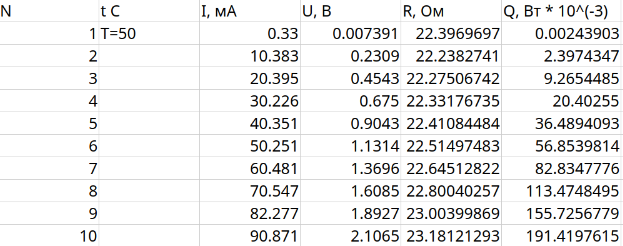
\includegraphics[width=0.6\textwidth]{tables/T50.png}
    \caption{Таблица с данными при $t = 50C^\circ$}
\end{figure}

\newpage

При $t = 60C^\circ$:
\begin{figure}[ht]
    \centering
    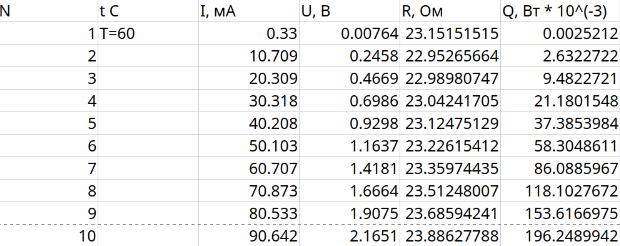
\includegraphics[width=0.6\textwidth]{tables/T60.png}
    \caption{Таблица с данными при $t = 60C^\circ$}
\end{figure}

При $t = 70C^\circ$:
\begin{figure}[ht]
    \centering
    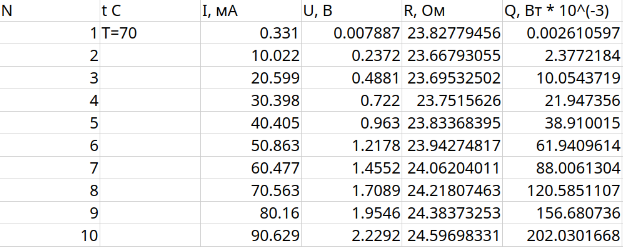
\includegraphics[width=0.6\textwidth]{tables/T70.png}
    \caption{Таблица с данными при $t = 70C^\circ$}
\end{figure}

Погрешности:\\

$\sigma_U = 0.003 \text{ В}$, \\

$\sigma_I = 0.003 \text{ мА}$, \\

$\frac{\sigma_Q}{Q} = \frac{\sigma_R}{R} = \sqrt{(\frac{\sigma_U}{U})^2 + (\frac{\sigma_I}{I})^2} \approx 0.01 = 1\%$.  \\

\subsection{Построение графиков $R(Q)$}

Для каждой температуры термостата построим график зависимости сопротивления нити от мощности $R(Q)$ и убедимся в линейности полученных
зависимостей. Проведём наилучшие прямые $y = kx + b$ и определим точки их пересечения с осью ординат $R_0$ (при $Q$ → 0 температура нити совпадает с температурой
термостата) и угловые коэффициенты наклона $\frac{dR}{dQ}$. \\

Погрешности:

$\sigma_k = \frac{1}{\sqrt{N}} \sqrt{\frac{<y^2> - <x><y>}{<x^2> - <x>^2} - b^2}$, \\

$\sigma_b = \sigma_k \sqrt{<x^2> - <x>^2}$, \\

$\frac{\sigma_{R_0}}{R_0} = \sqrt{(\frac{\sigma_R}{R})^2 + \sigma_b^2}$,  \\

$\frac{\sigma_{\frac{dR}{dQ}}}{\frac{dR}{dQ}} = \sqrt{(\frac{\sigma_R}{R})^2 + (\frac{\sigma_Q}{Q})^2 + \sigma_k^2}$.  \\

\newpage

При $t = 23C^\circ$:
\begin{figure}[ht]
    \centering
    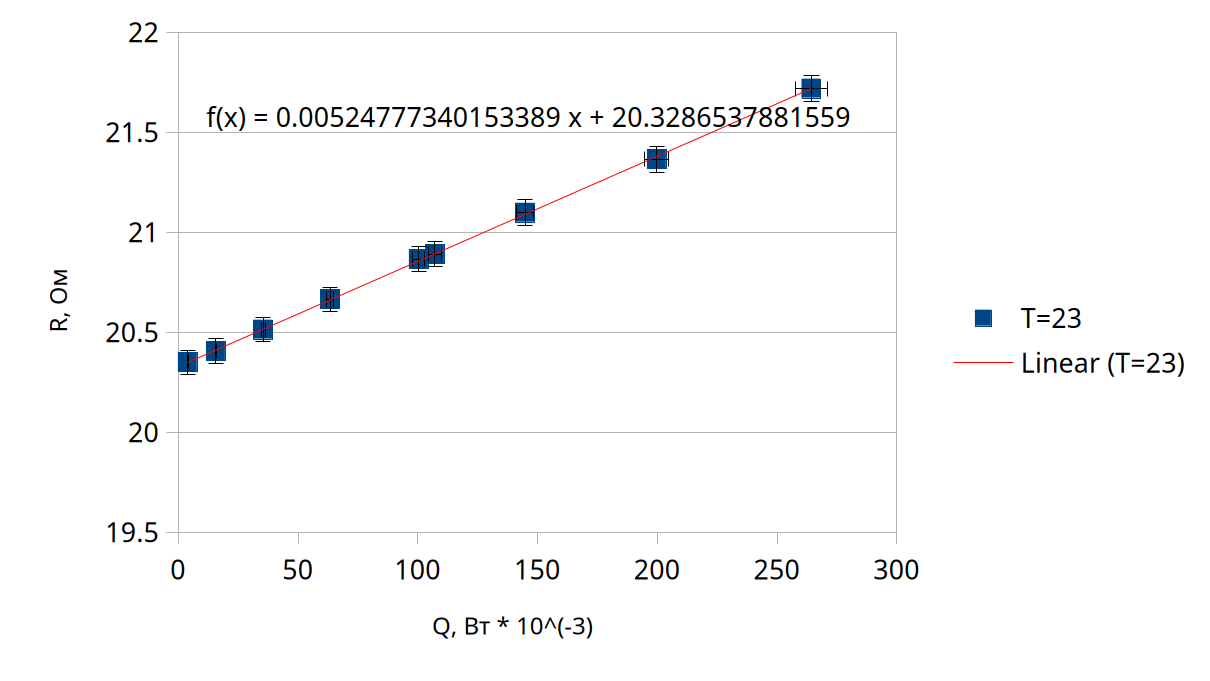
\includegraphics[width=0.7\textwidth]{charts_R_Q/T_23.png}
    \caption{График зависимости сопротивления нити $R$ от количества теплоты, выделяемой на ней при $t = 23C^\circ$}
\end{figure}

Получаем:
$R_0 = 20.33 \pm 0.02\text{ Ом}$,\\

$\frac{dR}{dQ} = (0.00524 \pm 0.00001) \cdot 10^3 \frac{\text{ Ом}}{\text{ Вт}}$. \\

%----------------------------------------------------------------------------------

При $t = 30C^\circ$:
\begin{figure}[ht]
    \centering
    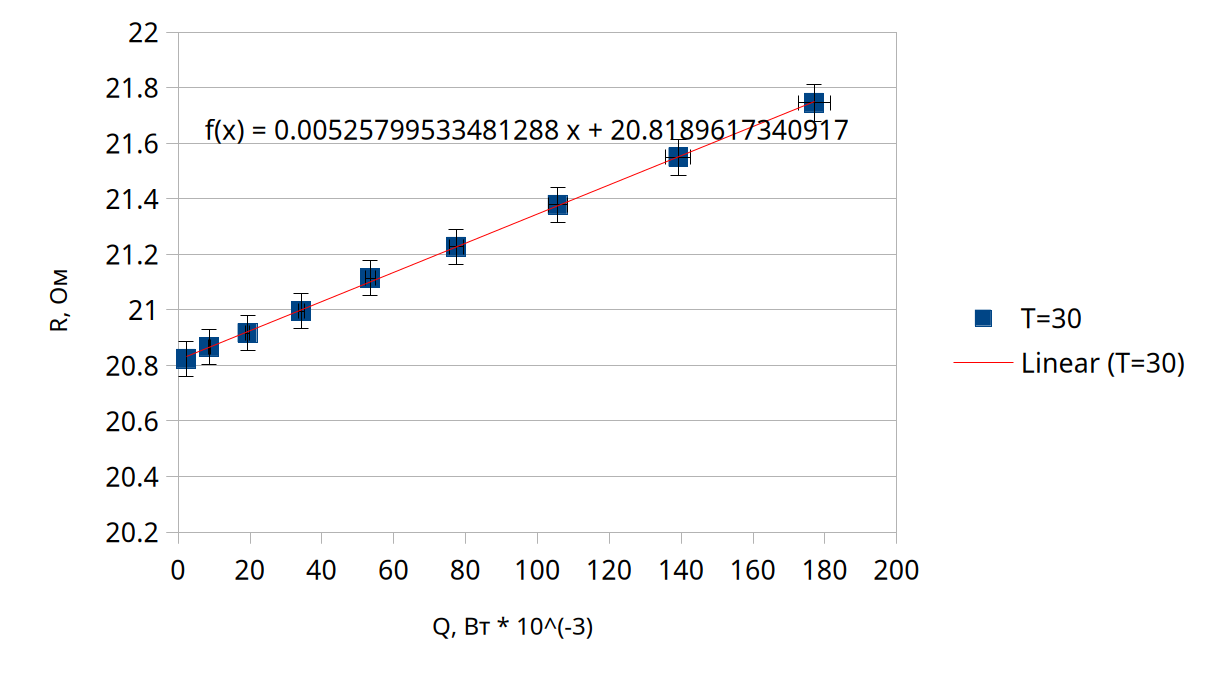
\includegraphics[width=0.7\textwidth]{charts_R_Q/T_30.png}
    \caption{График зависимости сопротивления нити $R$ от количества теплоты, выделяемой на ней при $t = 30C^\circ$}
\end{figure}

Получаем:
$R_0 = 20.82 \pm 0.02\text{ Ом}$,\\

$\frac{dR}{dQ} = (0.00526 \pm 0.00001) \cdot 10^3 \frac{\text{ Ом}}{\text{ Вт}}$. \\

%----------------------------------------------------------------------------------

При $t = 50C^\circ$:
\begin{figure}[ht]
    \centering
    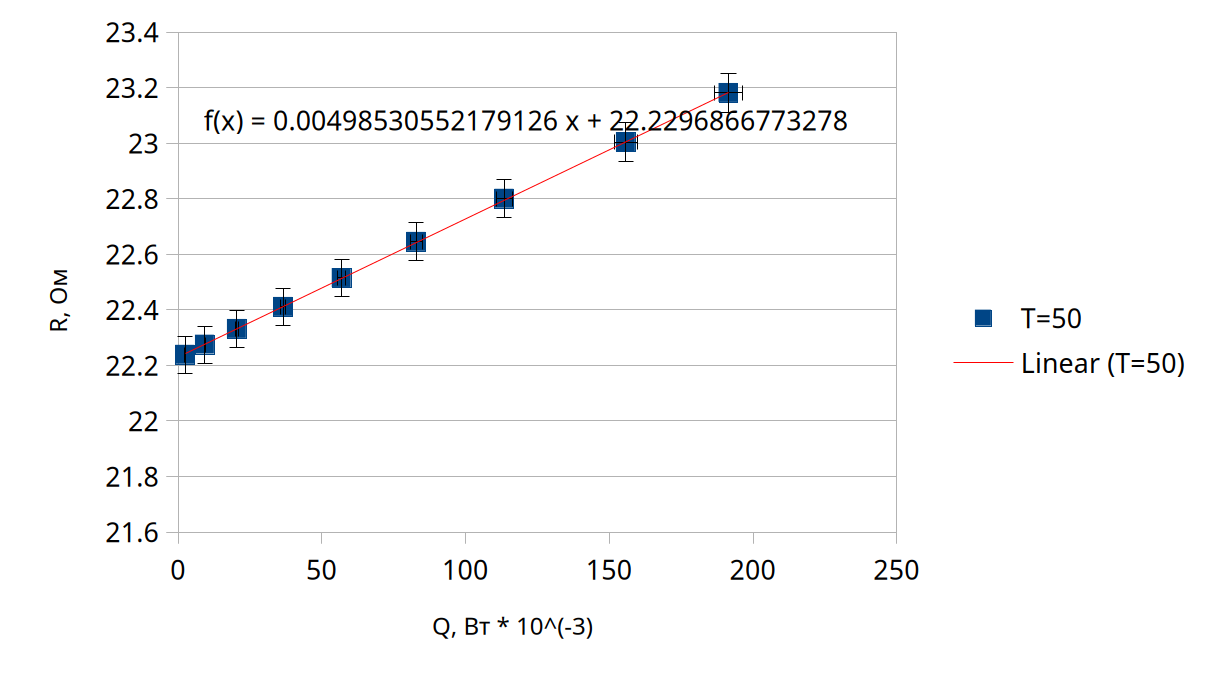
\includegraphics[width=0.7\textwidth]{charts_R_Q/T_50.png}
    \caption{График зависимости сопротивления нити $R$ от количества теплоты, выделяемой на ней при $t = 50C^\circ$}
\end{figure}

\newpage

Получаем:
$R_0 = 22.23 \pm 0.02\text{ Ом}$,\\

$\frac{dR}{dQ} = (0.00499 \pm 0.00001) \cdot 10^3 \frac{\text{ Ом}}{\text{ Вт}}$. \\

%----------------------------------------------------------------------------------

При $t = 60C^\circ$:
\begin{figure}[ht]
    \centering
    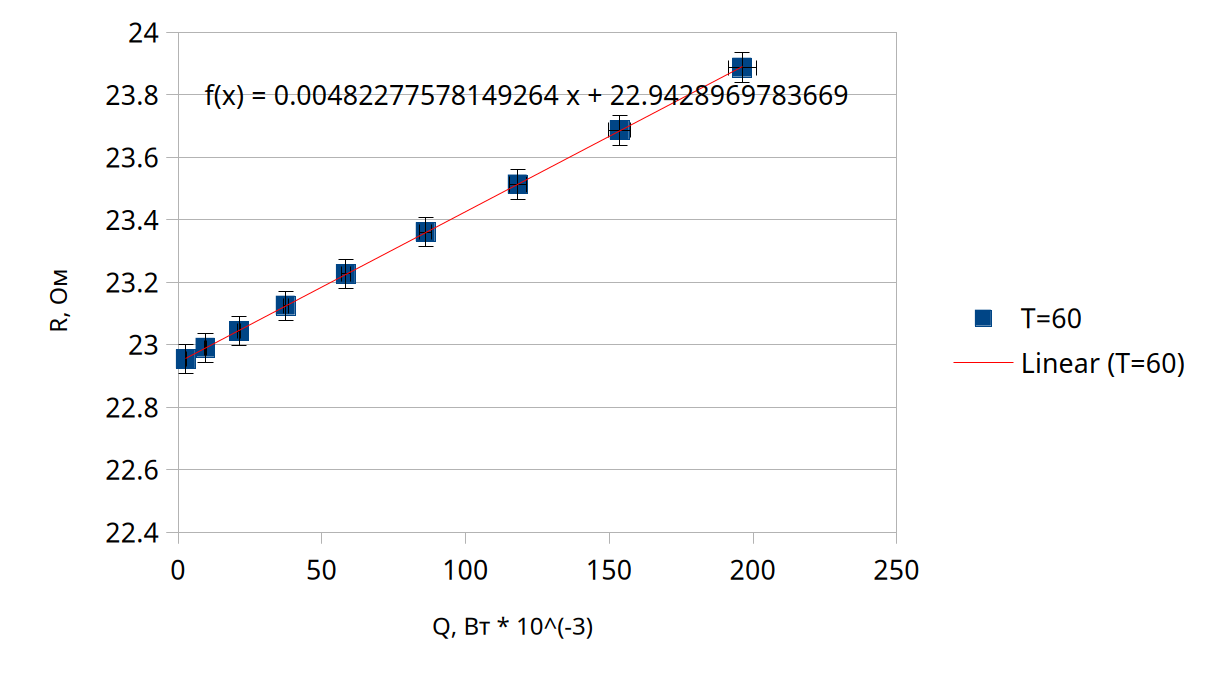
\includegraphics[width=0.7\textwidth]{charts_R_Q/T_60.png}
    \caption{График зависимости сопротивления нити $R$ от количества теплоты, выделяемой на ней при $t = 60C^\circ$}
\end{figure}

Получаем:
$R_0 = 22.94 \pm 0.02\text{ Ом}$,\\

$\frac{dR}{dQ} = (0.00482 \pm 0.00001) \cdot 10^3 \frac{\text{ Ом}}{\text{ Вт}}$. \\

%----------------------------------------------------------------------------------
\newpage

При $t = 70C^\circ$:
\begin{figure}[ht]
    \centering
    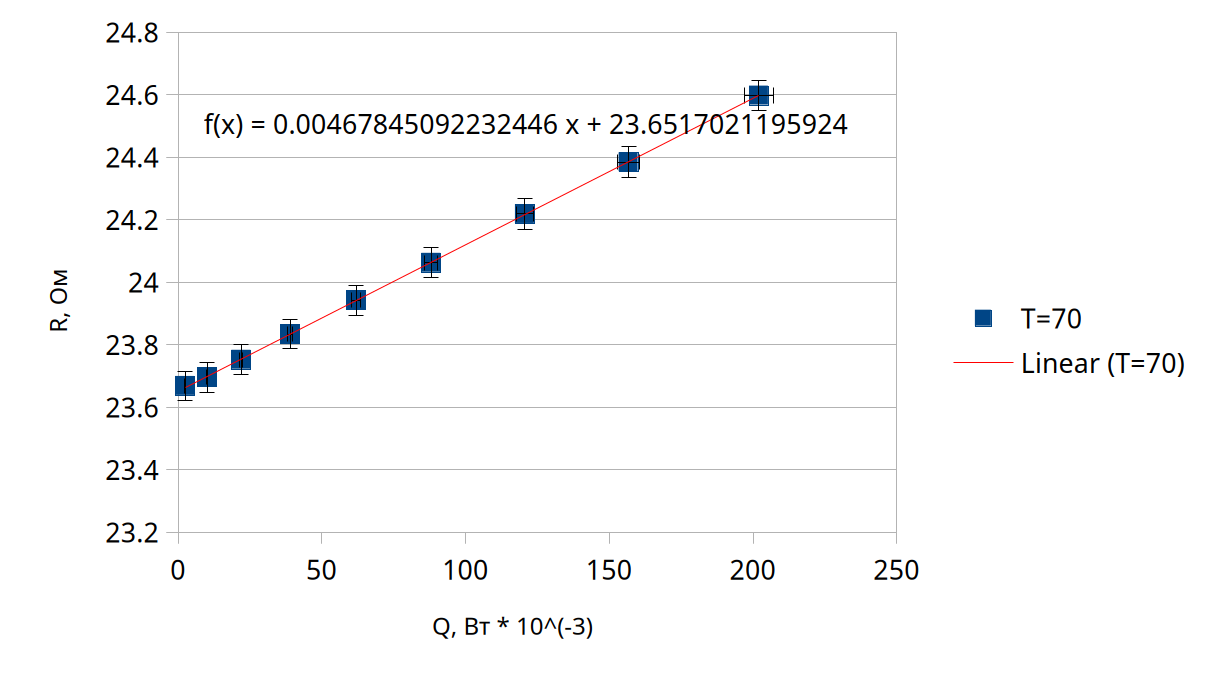
\includegraphics[width=0.7\textwidth]{charts_R_Q/T_70.png}
    \caption{График зависимости сопротивления нити $R$ от количества теплоты, выделяемой на ней при $t = 70C^\circ$}
\end{figure}

Получаем:
$R_0 = 23.65 \pm 0.02\text{ Ом}$,\\

$\frac{dR}{dQ} = (0.00468 \pm 0.00001) \cdot 10^3 \frac{\text{ Ом}}{\text{ Вт}}$. \\

%----------------------------------------------------------------------------------

\subsection{Построение графика $R_0(T)$}

По данным из предыдущего пункта построим график зависимости сопротивления проволки $R_0$ при его температуре $T$, совпадающей с температурой термостата, убедимся в линейности графика, проведём наилучшую прямую $y = kx + b$ и определим его угол наклона.

Погрешности:   \\

$\sigma_T = 0.03 \text{ K}$, \\

$\sigma_k = \frac{1}{\sqrt{N}} \sqrt{\frac{<y^2> - <x><y>}{<x^2> - <x>^2} - b^2}$, \\

$\frac{\sigma_{\frac{dR}{dT}}}{\frac{dR}{dT}} = \sqrt{(\frac{\sigma_{R_0}}{R_0})^2 + (\frac{\sigma_T}{T})^2 + \sigma_k^2}$. \\

Таблица с данными для графика:
\begin{figure}[ht]
    \centering
    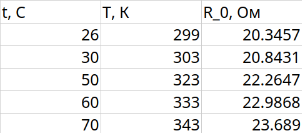
\includegraphics[width=0.4\textwidth]{R0_T/table_R0_T.png}
    \caption{Таблица с температурой термостата $T$ и сопроиивлением проволки при ней $R_0$}
\end{figure}

\newpage

График зависимости $R_0$ от $T$:

\begin{figure}[ht]
    \centering
    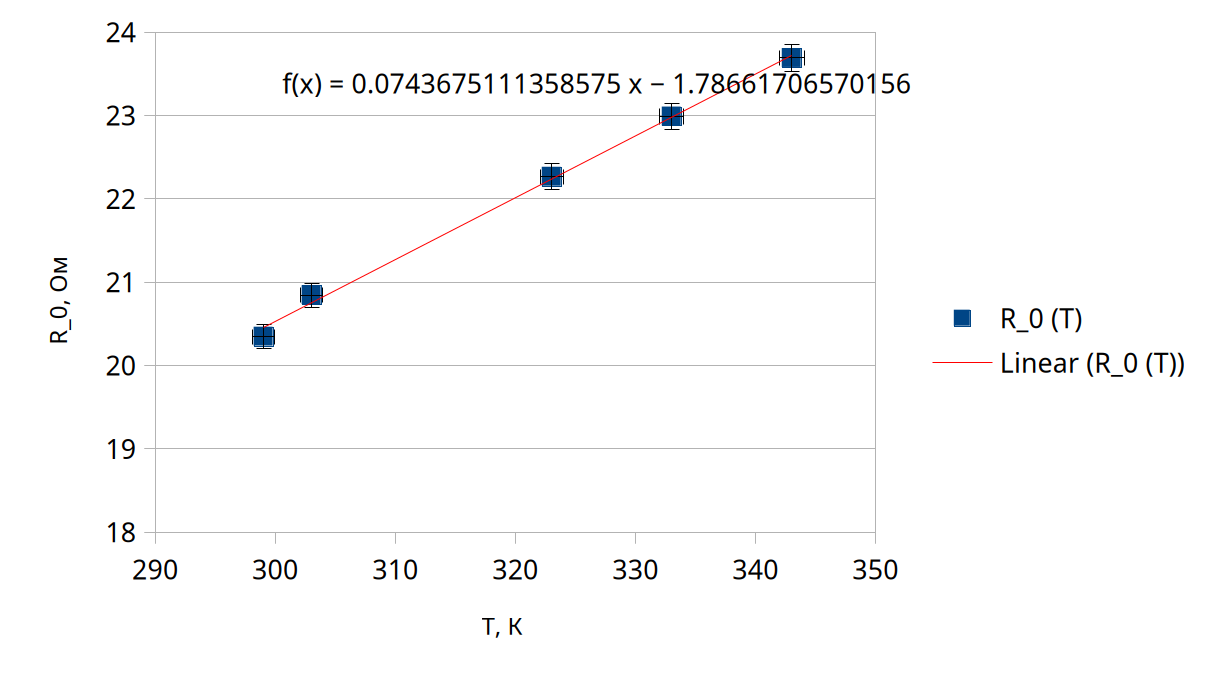
\includegraphics[width=0.7\textwidth]{R0_T/chart_R0_T.png}
    \caption{График зависимости сопротивления нити $R_0$ от температуры термостата $T$б совпадающей с температурой нити}
\end{figure}

Получаем:

$\frac{dR}{dT} = 0.074 \pm 0.002 \text{ }\frac{\text{Ом}}{K}$.

\subsection{Определение коэффициентов теплопроводности газа $k$ для каждой температуры термостата $T_0$}

\[\frac{dQ}{dT} = \frac{dR}{dT} / \frac{dR}{dQ} \],

\[k = \frac{dQ}{dT} \frac{1}{2\pi L} ln(\frac{r_2}{r_1})\]

Таблица со значениями $k$ при каждой $T$:

\begin{figure}[ht]
    \centering
    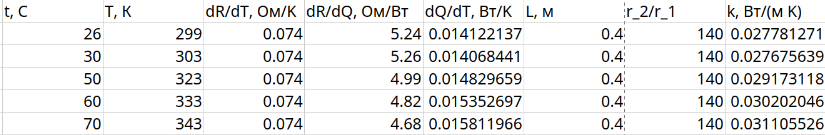
\includegraphics[width=0.7\textwidth]{k_T/table_k_T.png}
    \caption{Таблица со значениями коэффициентов теплопроводности
газа $k$ при каждой температуры термостата $T$}
\end{figure}

Данные коэффициентов теплопроводности газа $k$ сходятся с табличными ($\approx 0.025 \frac{\text{Вт}}{\text{м} \cdot K}$). \\

Погрешности: \\

$\sigma_k = \sqrt{(\frac{\sigma_{\frac{dR}{dT}}}{\frac{dR}{dT}})^2 + (\frac{\sigma_{\frac{dR}{dQ}}}{\frac{dR}{dQ}})^2}$.\\

\newpage

Из оценки графика зависимости $k$ от $T$, можно утверждать что эта зависмость приблизительно линейна:

 \begin{figure}[ht]
    \centering
    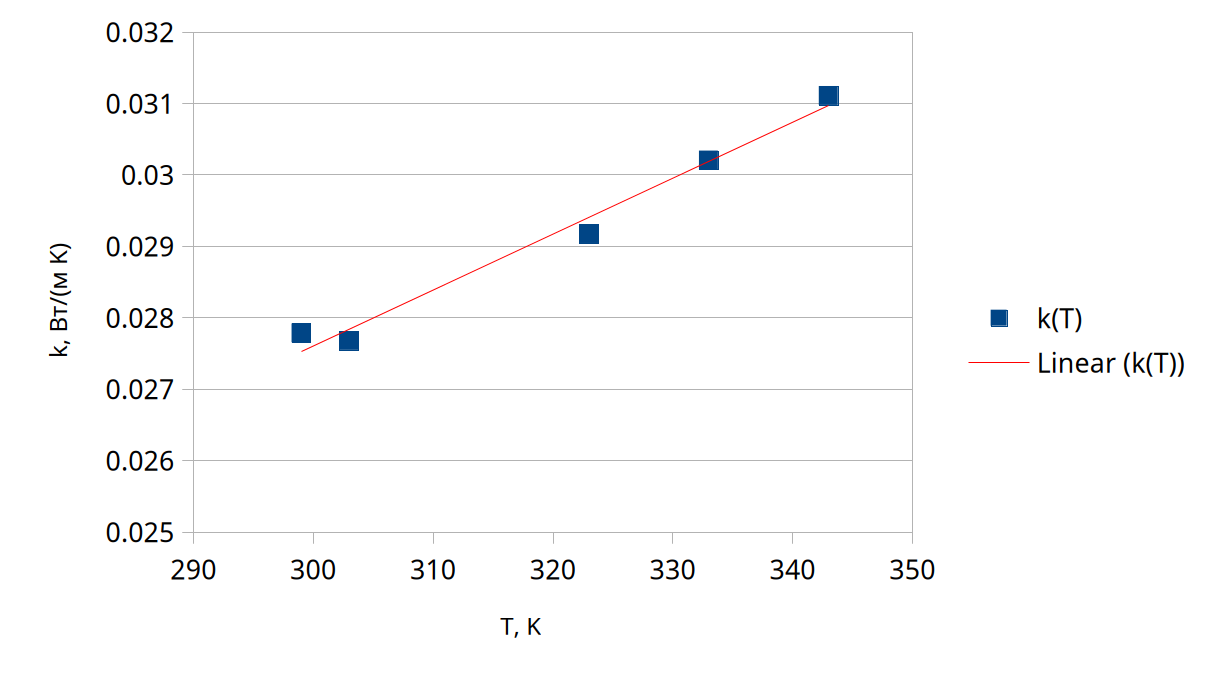
\includegraphics[width=0.7\textwidth]{k_T/chart_k_T.png}
    \caption{График зависимоти коэффициентов теплопроводности
газа $k$ при каждой температуры термостата $T$}
\end{figure}

\section{Вывод}

Мы измерили коэффициент теплопроводности воздуха при атмосферном
давлении в зависимости от температуры. Измерения совпали с табличными.


\end{document}

